% Options for packages loaded elsewhere
\PassOptionsToPackage{unicode}{hyperref}
\PassOptionsToPackage{hyphens}{url}
\PassOptionsToPackage{dvipsnames,svgnames,x11names}{xcolor}
%
\documentclass[
  ignorenonframetext,
]{beamer}
\usepackage{pgfpages}
\setbeamertemplate{caption}[numbered]
\setbeamertemplate{caption label separator}{: }
\setbeamercolor{caption name}{fg=normal text.fg}
\beamertemplatenavigationsymbolsempty
% Prevent slide breaks in the middle of a paragraph
\widowpenalties 1 10000
\raggedbottom
\setbeamertemplate{part page}{
  \centering
  \begin{beamercolorbox}[sep=16pt,center]{part title}
    \usebeamerfont{part title}\insertpart\par
  \end{beamercolorbox}
}
\setbeamertemplate{section page}{
  \centering
  \begin{beamercolorbox}[sep=12pt,center]{part title}
    \usebeamerfont{section title}\insertsection\par
  \end{beamercolorbox}
}
\setbeamertemplate{subsection page}{
  \centering
  \begin{beamercolorbox}[sep=8pt,center]{part title}
    \usebeamerfont{subsection title}\insertsubsection\par
  \end{beamercolorbox}
}
\AtBeginPart{
  \frame{\partpage}
}
\AtBeginSection{
  \ifbibliography
  \else
    \frame{\sectionpage}
  \fi
}
\AtBeginSubsection{
  \frame{\subsectionpage}
}
\usepackage{amsmath,amssymb}
\usepackage{lmodern}
\usepackage{iftex}
\ifPDFTeX
  \usepackage[T1]{fontenc}
  \usepackage[utf8]{inputenc}
  \usepackage{textcomp} % provide euro and other symbols
\else % if luatex or xetex
  \usepackage{unicode-math}
  \defaultfontfeatures{Scale=MatchLowercase}
  \defaultfontfeatures[\rmfamily]{Ligatures=TeX,Scale=1}
\fi
% Use upquote if available, for straight quotes in verbatim environments
\IfFileExists{upquote.sty}{\usepackage{upquote}}{}
\IfFileExists{microtype.sty}{% use microtype if available
  \usepackage[]{microtype}
  \UseMicrotypeSet[protrusion]{basicmath} % disable protrusion for tt fonts
}{}
\makeatletter
\@ifundefined{KOMAClassName}{% if non-KOMA class
  \IfFileExists{parskip.sty}{%
    \usepackage{parskip}
  }{% else
    \setlength{\parindent}{0pt}
    \setlength{\parskip}{6pt plus 2pt minus 1pt}}
}{% if KOMA class
  \KOMAoptions{parskip=half}}
\makeatother
\usepackage{xcolor}
\newif\ifbibliography
\usepackage{graphicx}
\makeatletter
\def\maxwidth{\ifdim\Gin@nat@width>\linewidth\linewidth\else\Gin@nat@width\fi}
\def\maxheight{\ifdim\Gin@nat@height>\textheight\textheight\else\Gin@nat@height\fi}
\makeatother
% Scale images if necessary, so that they will not overflow the page
% margins by default, and it is still possible to overwrite the defaults
% using explicit options in \includegraphics[width, height, ...]{}
\setkeys{Gin}{width=\maxwidth,height=\maxheight,keepaspectratio}
% Set default figure placement to htbp
\makeatletter
\def\fps@figure{htbp}
\makeatother
\setlength{\emergencystretch}{3em} % prevent overfull lines
\providecommand{\tightlist}{%
  \setlength{\itemsep}{0pt}\setlength{\parskip}{0pt}}
\setcounter{secnumdepth}{-\maxdimen} % remove section numbering
\usepackage{graphicx}
\usepackage{bm}
\usepackage{array}
\usepackage{amsmath}
\usepackage{amsthm}
\usepackage{amsfonts}
\usepackage{amssymb}
\usepackage{tikz-cd}
\usepackage{url}
\definecolor{foreground}{RGB}{255,255,255}
\definecolor{background}{RGB}{34,28,54}
\definecolor{title}{RGB}{105,165,255}
\definecolor{gray}{RGB}{175,175,175}
\definecolor{lightgray}{RGB}{225,225,225}
\definecolor{subtitle}{RGB}{232,234,255}
\definecolor{hilight}{RGB}{112,224,255}
\definecolor{vhilight}{RGB}{255,111,207}
\setbeamertemplate{footline}[page number]
\ifLuaTeX
  \usepackage{selnolig}  % disable illegal ligatures
\fi
\IfFileExists{bookmark.sty}{\usepackage{bookmark}}{\usepackage{hyperref}}
\IfFileExists{xurl.sty}{\usepackage{xurl}}{} % add URL line breaks if available
\urlstyle{same} % disable monospaced font for URLs
\hypersetup{
  pdftitle={STAT 528 - Advanced Regression Analysis II},
  pdfauthor={Exponential family theory (part 3)},
  colorlinks=true,
  linkcolor={Maroon},
  filecolor={Maroon},
  citecolor={Blue},
  urlcolor={blue},
  pdfcreator={LaTeX via pandoc}}

\title{STAT 528 - Advanced Regression Analysis II}
\author{Exponential family theory (part 3)}
\date{}
\institute{Daniel J. Eck\\
Department of Statistics\\
University of Illinois}

\begin{document}
\frame{\titlepage}

\begin{frame}
\newcommand{\R}{\mathbb{R}}
\newcommand{\Prob}{\mathbb{P}}
\newcommand{\Proj}{\textbf{P}}
\newcommand{\Hcal}{\mathcal{H}}
\newcommand{\rootn}{\sqrt{n}}
\newcommand{\p}{\mathbf{p}}
\newcommand{\E}{\text{E}}
\newcommand{\Var}{\text{Var}}
\newcommand{\Cov}{\text{Cov}}

\newtheorem{cor}{Corollary}
\newtheorem{lem}{Lemma}
\newtheorem{thm}{Theorem}
\newtheorem{defn}{Definition}
\newtheorem{prop}{Proposition}
\end{frame}

\begin{frame}{Last time}
\protect\hypertarget{last-time}{}
\begin{itemize}
\tightlist
\item
  mean value parameters
\item
  maximum likelihood estimation (MLE)
\item
  asymptotics of MLE
\item
  finite sample concentration of MLE
\end{itemize}
\end{frame}

\begin{frame}{Learning Objectives Today}
\protect\hypertarget{learning-objectives-today}{}
\begin{itemize}
\tightlist
\item
  generalized linear models (GLMs)
\item
  different parameterizations
\end{itemize}
\end{frame}

\begin{frame}{Canonical linear submodels: intro to GLMs}
\protect\hypertarget{canonical-linear-submodels-intro-to-glms}{}
We now motivate generalized linear models (GLMs) within the context of
exponential theory.

A canonical affine submodel of an exponential family is a submodel
having parameterization \[
  \theta = a + M\beta
\] where:

\begin{itemize}
\tightlist
\item
  \(\theta \in \mathbb{R}^n\) is the canonical parameter vector
\item
  \(\beta \in \mathbb{R}^p\) is the canonical parameter vector for the
  submodel
\item
  \(a \in \mathbb{R}^n\) is a known offset vector
\item
  \(M \in \mathbb{R}^{n\times p}\) is a known \emph{model matrix}.
\end{itemize}
\end{frame}

\begin{frame}{}
\protect\hypertarget{section}{}
In most applications the offset vector is not used giving
parameterization \[
  \theta = M\beta,
\]\\
in which case we say the submodel is a \emph{canonical linear submodel}.

We will restrict attention to the canonical linear submodel in this
class.
\end{frame}

\begin{frame}{}
\protect\hypertarget{section-1}{}
The canonical linear submodel log likelihood is given by
\begin{equation} \label{subloglike}
\begin{split}
  l(\theta) &= \langle y,\theta\rangle - c(\theta) \\
    &= \langle y,M\beta\rangle - c(M\beta) \\
    &= \langle M'y,\beta\rangle - c_\beta(\beta),   
\end{split}
\end{equation} and we see that we again have an exponential family with

\begin{itemize}
\tightlist
\item
  canonical statistic \(M'y\)
\item
  cumulant function \(\beta \mapsto c_\beta(\beta) = c(M\beta)\)
\item
  submodel canonical parameter vector \(\beta\)
\end{itemize}
\end{frame}

\begin{frame}{}
\protect\hypertarget{section-2}{}
Let's step back a bit.

In applications \(n\) denotes the sample size.
\(\theta \in \mathbb{R}^n\) is an arbitrary vector specifying one
parameter for individual. This is a saturated model.

For a model to be useful, we need dimension reduction \[
  \theta = M\beta.
\] In other words, \(\theta \in \text{span}(M)\).
\end{frame}

\begin{frame}{Full regular submodels}
\protect\hypertarget{full-regular-submodels}{}
If the originally given full canonical parameter space was \(\Theta\),
then the full submodel canonical parameter space is \[
  B = \{\beta : M\beta \in \Theta\}.
\]

Thus a canonical linear submodel gives us a new exponential family, with
lower-dimensional canonical parameter and statistic.

The submodel exponential family is full regular if the original
exponential family was full regular.
\end{frame}

\begin{frame}{Parameterizations}
\protect\hypertarget{parameterizations}{}
Now we have four parameters:

\begin{itemize}
\tightlist
\item
  the saturated model canonical and mean value parameters \(\theta\) and
  \(\mu\)
\item
  the canonical linear submodel canonical and mean value parameters
  \(\beta\) and \(\tau = M^T\mu\).
\end{itemize}

The observed equals expected property for the submodel is
\begin{equation} \label{submodelmvp}
    \hat\tau = M^T\hat\mu = M^Ty.
\end{equation}
\end{frame}

\begin{frame}{}
\protect\hypertarget{section-3}{}
A depiction of the transformations necessary to change between
parameterizations.

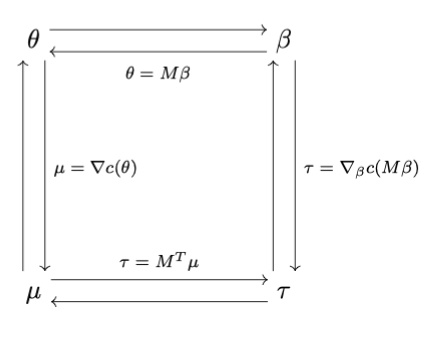
\includegraphics{transformations.png}
\end{frame}

\begin{frame}{}
\protect\hypertarget{section-4}{}
\textbf{Note}: \(\mu \to M^T\mu\) is usually not one-to-one (when
\(n > p\) and \(M\) is full column rank).

Hence we cannot determine \(\hat\theta\) and \(\hat\beta\) from them
either.

The only way to determine the MLEs is to maximize the log likelihood
\eqref{subloglike} to obtain \(\hat\beta\) and then

\begin{itemize}
\tightlist
\item
  \(\hat\theta = M\hat\beta\)
\item
  \(\hat\mu = \nabla c(\hat\theta)\)
\item
  \(\hat\tau = M^T\hat\mu\).
\end{itemize}
\end{frame}

\begin{frame}{GLMs and link functions}
\protect\hypertarget{glms-and-link-functions}{}
Recall that the saturated model canonical parameter vector \(\theta\) is
\emph{linked} to the saturated model mean value parameter vector through
the change-of-parameter mappings \(g(\theta)\).

We can reparameterize \(\theta = M\beta\) and write \[
 \mu = \text{E}_\theta(Y) = g(M\beta) 
\] which implies that we can write \[
  g^{-1}\left(\text{E}_\theta(Y)\right) = M\beta.
\]
\end{frame}

\begin{frame}{}
\protect\hypertarget{section-5}{}
Therefore, a linear function of the canonical submodel parameter vector
is linked to the mean of the exponential family through the inverse
change-of-parameter mapping \(g^{-1}\).

This is the basis of exponential family generalized linear models with
link function \(g^{-1}\).

Note that most treatments of GLMs will present \(g^{-1}\) as the link
function. Instead we motivated a change of parameters mapping from
canonical to mean value parameters.
\end{frame}

\begin{frame}{Example: logistic regression}
\protect\hypertarget{example-logistic-regression}{}
Let \(M\) have rows \(x_i'\), \(i = 1\), \(\ldots\), \(n\). Then
\(\theta_i = x_i'\beta\) and

\[
  x_i'\beta = \log\left(\frac{p_i}{1 - p_i}\right) \qquad \text{and} \qquad p_i = \left(\frac{\exp(x_i'\beta)}{ 1 + \exp(x_i'\beta)}\right),
\] where \begin{align*}
  &\sum_{i=1}^n\left[y_i\log(p_i) - (1 - y_i)\log(p_i) \right]
   = \sum_{i=1}^n\left[y_ix_i'\beta - \log(1 + \exp(x_i'\beta))\right] \\
    &= \sum_{i=1}^n\left[\langle y_i, x_i'\beta \rangle - \log(1 + \exp(x_i'\beta)) \right] \\
    &= \langle y, \theta \rangle - \sum_{i=1}^n \log(1 + \exp(\theta_i)) \\
    &= \langle y, \theta \rangle - c(\theta). \\
\end{align*}
\end{frame}

\begin{frame}{}
\protect\hypertarget{section-6}{}
Alternatively, \begin{align*}
  &\sum_{i=1}^n\left[\langle y_i, x_i'\beta \rangle - \log(1 + \exp(x_i'\beta)) \right] \\
  &= \langle \sum_{i=1}^n y_i x_i, \beta \rangle - \sum_{i=1}^n\log(1 + \exp(x_i'\beta)) \\
  &= \langle M'y, \beta \rangle - c_\beta(\beta)  
\end{align*}
\end{frame}

\end{document}
